\documentclass[a1]{sciposter}
\usepackage{epsfig}
\usepackage{amsmath}
\usepackage{amssymb}
\usepackage{multicol}
\usepackage{graphicx,url}
\usepackage[portuges, brazil]{babel}   
\usepackage[utf8]{inputenc}
\usepackage[sfdefault]{FiraSans} 
\usepackage{inconsolata}
\usepackage[T1]{fontenc}
\renewcommand*\oldstylenums[1]{{\firaoldstyle #1}}
\usepackage[cm]{sfmath}
\usepackage{tcolorbox}
\usepackage{xcolor}
%\usepackage{fancybullets}
\usepackage{subfig}
\usepackage{graphicx}
\usepackage[round,sort,nonamebreak]{natbib}
\setcitestyle{open={[},close={]}}
\newtheorem{Def}{Definition}

\newcommand\kcont{\protect\mathpalette{\protect\independenT}{\perp}}
\def\independenT#1#2{\mathrel{\rlap{$#1#2$}\mkern2mu{#1#2}}}

\newcommand{\krev}{\downarrow\downarrow}

% create subfigure environment
\def\subfigure{\let\oldcaption=\caption
\let\caption=\subcaption
\minipage}
\def\endsubfigure{\endminipage
\let\caption=\oldcaption}

\newcommand{\subcaption}[1]% %1 = text
{\refstepcounter{subfig}%
\par\vskip\abovecaptionskip
\centerline{\textbf{(\alph{subfig})} #1}%
\vskip\belowcaptionskip\par}

\urlstyle{same}

\title{Filtragem de Ruído Telúrico em Sinais Astronômicos}
%Título do projeto

\author{
Isabela Blücher \\
Orientadora: Prof.ª Dra. Paula Rodrigues Teixeira Coelho (IAG)\\
Coorientador: Prof. Dr. Marcelo Gomes de Queiroz\\}
%nome dos autores

\institute 
{Instituto de Matemática e Estatística \\
 Universidade de São Paulo}
%Nome e endereço da Instituição

% \email{isabela.blucher@usp.br}
% Onde você coloca os emails dos integrantes

\rightlogo[1.2]{usp-logo-png}
\leftlogo[1]{ime}
% Exibe os logos (direita e esquerda) 
% Procure usar arquivos png ou jpg, e de preferencia mantenha na mesma pasta do .tex
%%%%%%%%%%%%%%%%%%%%%%%%%%%%%%%%%%%%%%%%%%%%%%%%%%%%%%%%%%%%%%%%%%%%%%%%%%%%%%%%
%%% Begin of Document

\begin{document}
%define conference poster is presented at (appears as footer)

%\LEFTSIDEfootlogo  
% Uncomment to put footer logo on left side, and 
% conference name on right side of footer

% Some examples of caption control (remove % to check result)

%\renewcommand{\algorithmname}{Algoritme} % for Dutch

%\renewcommand{\mastercapstartstyle}[1]{\textit{\textbf{#1}}}
%\renewcommand{\algcapstartstyle}[1]{\textsc{\textbf{#1}}}
%\renewcommand{\algcapbodystyle}{\bfseries}
%\renewcommand{\thealgorithm}{\Roman{algorithm}}

\maketitle

%%% Begin of Multicols-Enviroment
\begin{multicols}{2}

%%% Abstract
\Section{Introdução}

Estrelas emitem energia na forma de radiação eletromagnética. Para capturar este sinal a partir do solo, são utilizados espectrógrafos, instrumentos de observação que produzem espectros: mapas da radiação em função do comprimento de onda.\\

Antes da captura do espectro, a atmosfera terrestre interage com a radiação da estrela, o que resulta em um espectro observado distorcido e contaminado, devido à formação de novas linhas no espectro, denominadas linhas telúricas.\\

Neste trabalho foram estudados métodos existentes de correção telúrica e potenciais soluções computacionais que sejam capazes de remover ou atenuar a contaminação telúrica de espectros estelares capturados a partir do solo.

\Section{Contaminação Telúrica}

Em termos matemáticos, o problema da contaminação telúrica pode ser descrito como: consideramos os vetores $o$ (observado), $a$ (atmosfera) e $s$ (estrela), que representam os espectros observado, telúrico e estelar sem contaminação. Podemos representar a contaminação telúrica pela equação
\begin{equation*}
    o = a \circ s \qquad \left(\mbox{ou equivalentemente:} \qquad o_i = a_i\cdot s_i,\ \forall i\right).
\end{equation*}

Devido à natureza multiplicativa do problema, a correção telúrica dos espectros observados seria a divisão simples do espectro observado pelo telúrico. Porém, esta formulação do problema pressupõe que as três sequências estão perfeitamente alinhadas, o que não corresponde à realidade.

\Section{Correção Telúrica}

Foi feito um experimento para testar o método da correção telúrica pela divisão simples dos espectros, de modo a observar que na prática esta solução não é ideal e cria artefatos no espectro estelar observado.

\begin{figure}
 \centering
 \begin{subfigure}{0.4\textwidth}
  \centering
  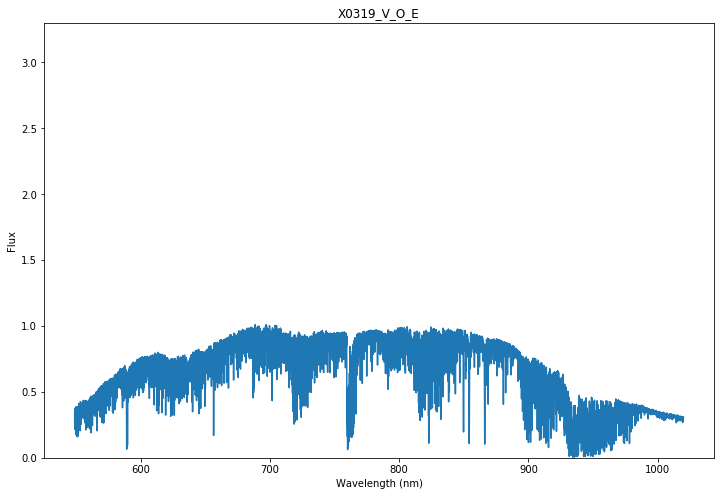
\includegraphics[width=1.1\textwidth]{x0319_v_o_e_scaled.png}
  \caption{X0319}
 \end{subfigure}\hfil
 \begin{subfigure}{0.4\textwidth}
  \centering
  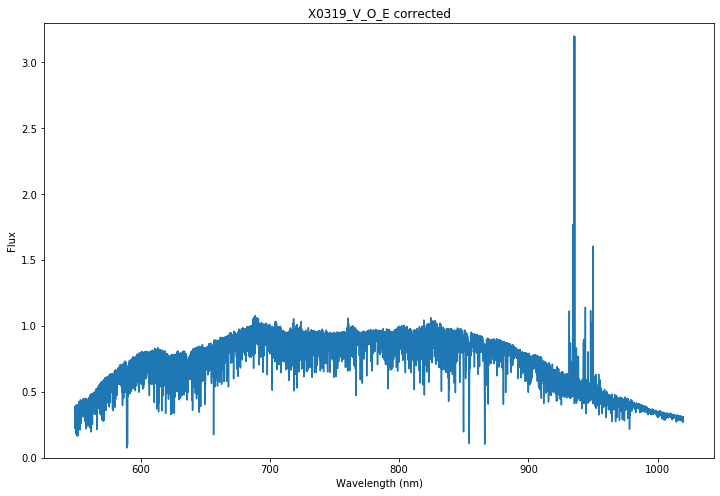
\includegraphics[width=1.1\textwidth]{x0319_v_o_e_divided.png}
  \caption{Correção telúrica de X0319}
 \end{subfigure}\hfil
%   \caption{fig}
\end{figure}

A divisão da estrela X0319 \cite{Chen2014TheXS} por seu referencial telúrico correspondente ilustra as dificuldades deste método de correção telúrica. São observados picos no sinal que não deveriam existir na situação ideal do problema. Este resultado indica a presença de um desalinhamento entre o espectro estelar e o telúrico \cite{unpublished-xshooter-data-release}.

\Section{Aplicação do \textit{Dynamic Time Warping}}

Uma proposta para melhorar a qualidade da correção telúrica do trabalho foi realinhar o espectro telúrico em relação ao estelar. A abordagem selecionada para isso foi o algoritmo \textit{Dynamic Time Warping}. Este algoritmo encontra uma correspondência entre os índices de dois vetores de modo a minimizar as distâncias entre estes índices.

\begin{figure}
 \centering
 \begin{subfigure}{0.4\textwidth}
  \centering
  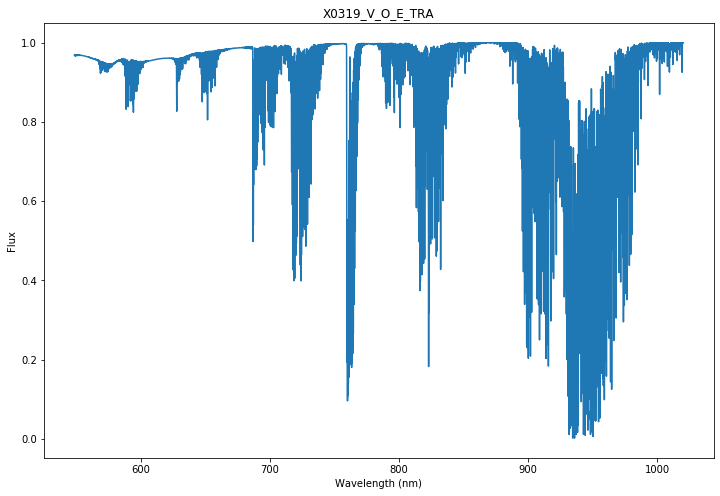
\includegraphics[width=1.1\textwidth]{x0319_v_o_e_tra.png}
  \caption{Modelo telúrico X0319}
 \end{subfigure}\hfil
 \begin{subfigure}{0.4\textwidth}
  \centering
  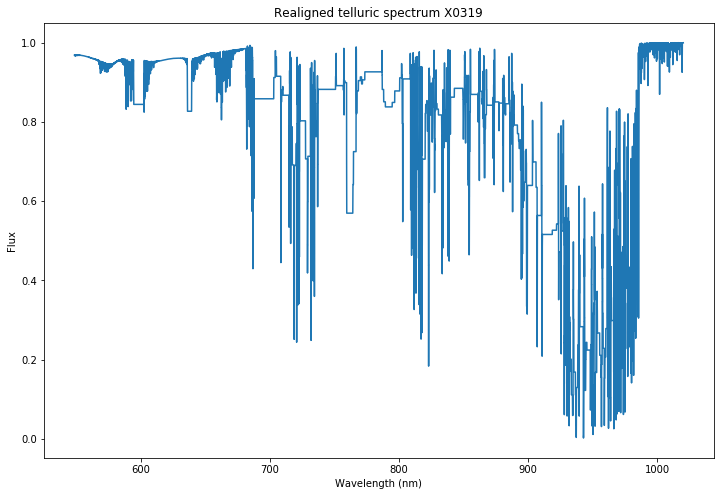
\includegraphics[width=1.1\textwidth]{x0319_v_o_e_aligned.png}
  \caption{Telúrico realinhado X0319}
 \end{subfigure}\hfil
%   \caption{fig}
\end{figure}

A aplicação do DTW como método de realinhamento criou ruídos no dado espectral. Por mais que o espectro telúrico realinhado da estrela X0319 \cite{Chen2014TheXS} tenha grosso modo um perfil compatível com o obtido por simuladores, ele possui uma forte distorção em relação às linhas espectrais originais e exibe a formação de ângulos retos que não são característicos deste tipo de dado. \\

Uma hipótese para explicar o baixo desempenho da aplicação do DTW nos espectros completos seriam as grandes diferenças de perfil global que se observam entre eles. O próximo experimento selecionado foi testar o algoritmo de realinhamento em regiões menores do espectro.

\begin{figure}
 \centering
 \begin{subfigure}{0.4\textwidth}
  \centering
  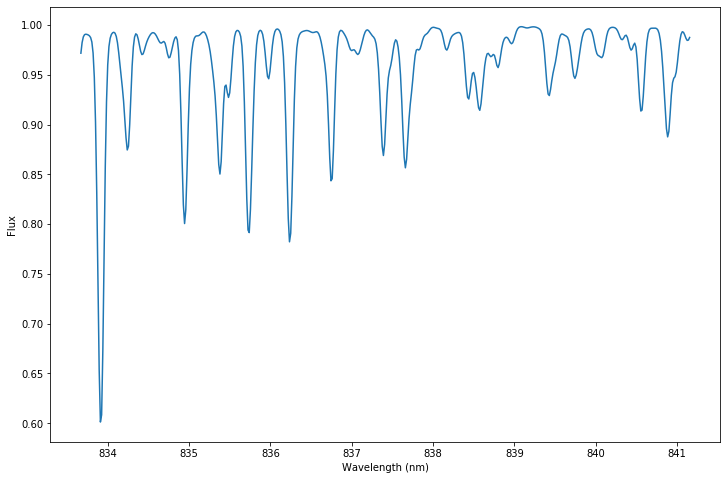
\includegraphics[width=1.1\textwidth]{x0319_v_o_e_tra_zoom.png}
  \caption{Zoom modelo telúrico X0319}
 \end{subfigure}\hfil
 \begin{subfigure}{0.4\textwidth}
  \centering
  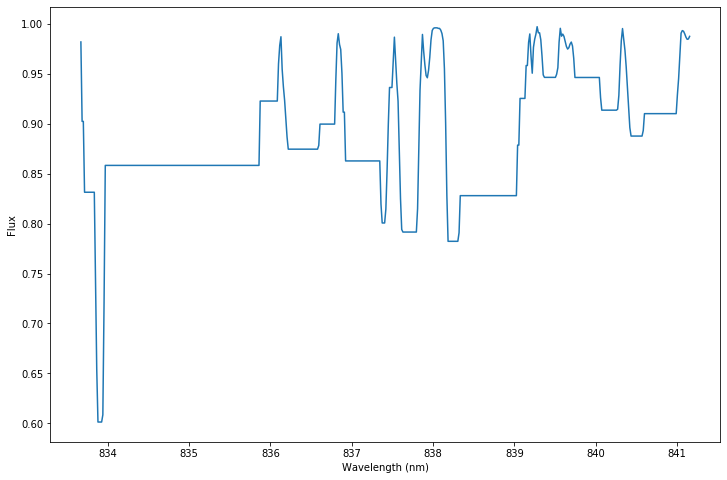
\includegraphics[width=1.1\textwidth]{x0319_v_o_e_aligned_zoom.png}
  \caption{Zoom telúrico realinhado X0319}
 \end{subfigure}\hfil
%   \caption{fig}
\end{figure}

Neste intervalo menor de 9nm do espectro telúrico de X0319 \cite{Chen2014TheXS}, ocorre a mesma formação de ângulos retos nas linhas de absorção. Isto indica que o DTW não produz alinhamentos razoáveis quando aplicado em sinais que não representam a mesma informação, ainda que possuam linhas de absorção comuns.\\

Usando dados de pesquisadores \cite{unpublished-xshooter-data-release} que fizeram correções manuais nos desalinhamentos nos espectros estelares, foi possível reconstruir o espectro telúrico \textit{ground-truth} para este trabalho. Desta forma, se temos os vetores $o$ e $c$ que representam a observação contaminada e o espectro final corrigido, teríamos o espectro real de transmitância da atmosfera dado por
\begin{equation*}
    a' = o \oslash c \qquad \left(\mbox{ou equivalentemente:} \qquad a'_{i} = o_i / c_i,\ \forall i\right),
\end{equation*}

assim é possível compará-lo com o sinal atmosférico obtido com o conjunto de dados do XSL \cite{Chen2014TheXS}.

\begin{figure}
 \centering
 \begin{subfigure}{0.4\textwidth}
  \centering
  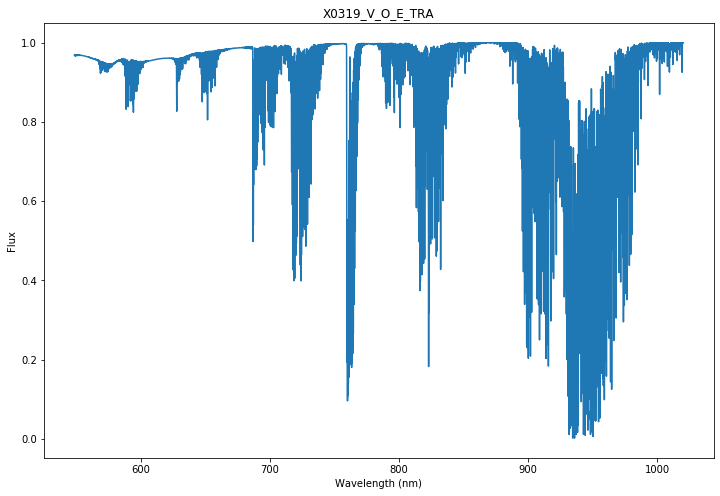
\includegraphics[width=1.1\textwidth]{x0319_v_o_e_tra.png}
  \caption{Modelo telúrico X0319}
 \end{subfigure}\hfil
 \begin{subfigure}{0.4\textwidth}
  \centering
  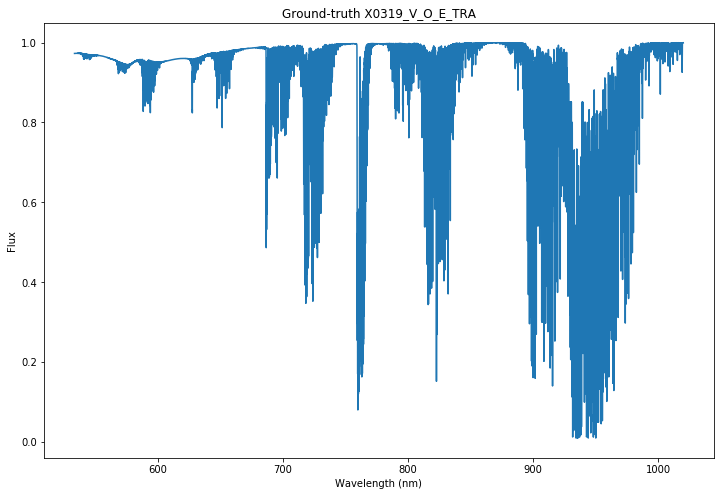
\includegraphics[width=1.1\textwidth]{x0319_v_o_e_tra_gt.png}
  \caption{Telúrico \textit{ground-truth} X0319}
 \end{subfigure}\hfil
%   \caption{fig}
\end{figure}

Estas figuras ilustram que é possível aplicar o DTW em dados que representam duas versões desalinhadas da mesma informação.

\Section{Conclusões}

A abordagem escolhida para melhorar a qualidade da correção telúrica tinha como objetivo explorar as linhas de absorção em comum entre o espectro observado e o espectro telúrico. Os experimentos mostram que o algoritmo DTW não é ideal para esta aplicação, visto que ele distorce o espectro telúrico para minimizar a distância à referência estelar observada, o que não corresponde a uma solução generalizável para observações estelares e seus referenciais telúricos. 

% \bibliography{bibliografia}
%%% References

%% Note: use of BibTeX als works!!

\bibliographystyle{plain}
\bibliography{bibliografia}

\end{multicols}

\end{document}